\subsection{User Interface}	
	\subsubsection{Mission control interface design} %Wenkai
	\noindent
The user interface is an integrated development environment, it is a graphical application written in C\#, it allows the user to drag the mission from the missions panel and drop them to the painting panel, use straight line arrow or a curve line arrow to connect the missions. It also includes the PID control setting part and CAN message control part, all the output from this interface are JSON strings.

The flowchart that in fig. \ref{IDE_overall_design} show the whole design of the user interface. First finish the drag-and-drop part, second make use arrow to connect with the node come true, finish the JSON string output through the TCP communication.
\begin{figure}[!ht]
	\begin{center}
		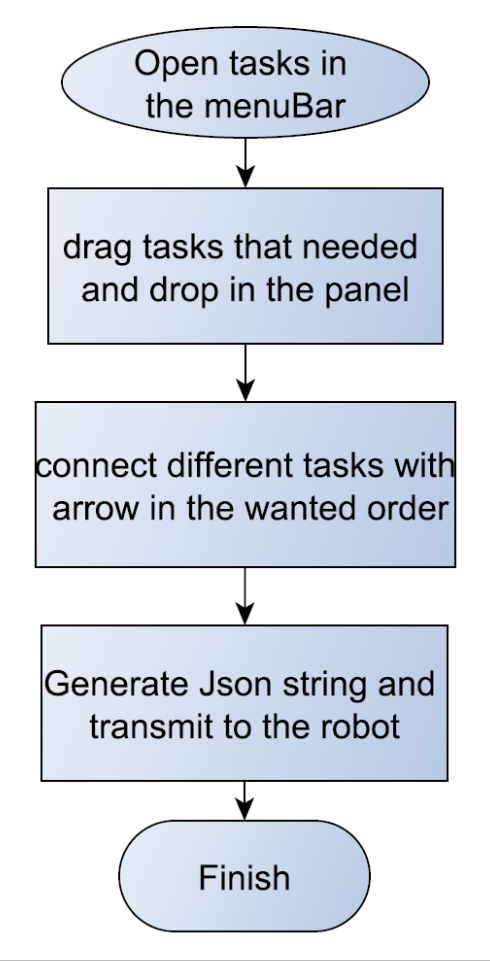
\includegraphics[width=50mm]{./Images/Software/IDE_overall_design.png}
		\caption{IDE over all design flowchart}
		\label{IDE_overall_design}
	\end{center}
\end{figure}

The drag and drop part mainly use the Microsoft Visual Studio tool, the drag part use the toolStrip bar which is a develop tool you can drag button from it easily. The drop part use the painting panel which you can drop some components on it. If there is a task or an arrow was dropped on the panel, then this component is added to the PaintItem List<>. The purpose of doing this is to make sure it is easy to manage all the items on the panel, then the painting panel will trigger the onPaintBackground and onPaint method, so the panel will refresh and repaint. The flowchart that in fig. \ref{drag_drop_design} is the design flowchart for the drag and drop event part.
\begin{figure}[!ht]
	\begin{center}
		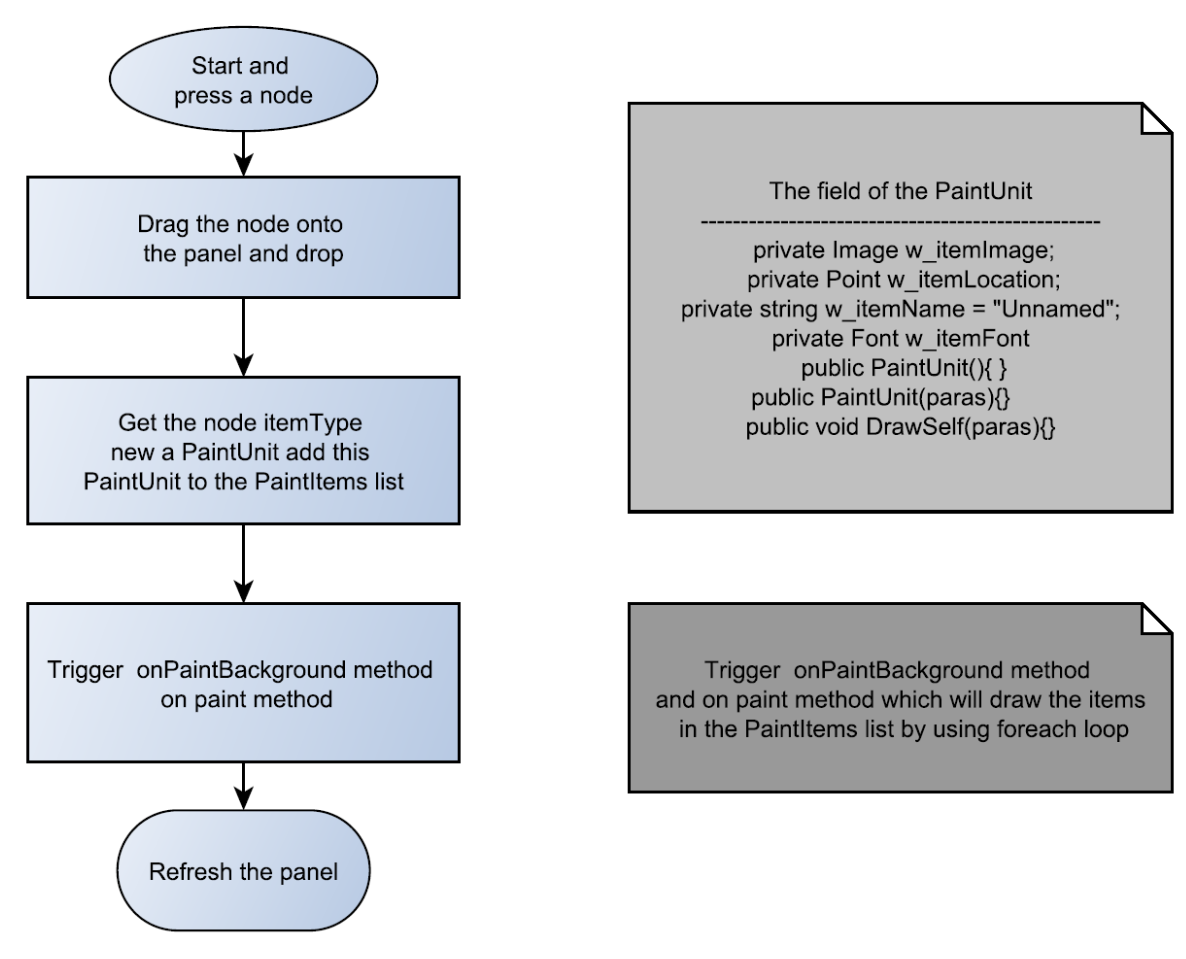
\includegraphics[width=80mm]{./Images/Software/drag_drop_design.png}
		\caption{The drag and drop design flowchart of IDE}
		\label{drag_drop_design}
	\end{center}
\end{figure} 
After dropping a task on the panel, the node should still be moveable. When click the mouse, the first thing need to do is to check which side of the mouse was pressed, if it was left button, then set the move value equal to true and get the start position of the node, calculate how far did the mouse move and set the new coordinate equal to the node, refresh the paint panel and set the move value equal to false. The flowchart that in fig. \ref{drag_button_on_panel} is the drag node move on the panel design.
\begin{figure}[!ht]
	\begin{center}
		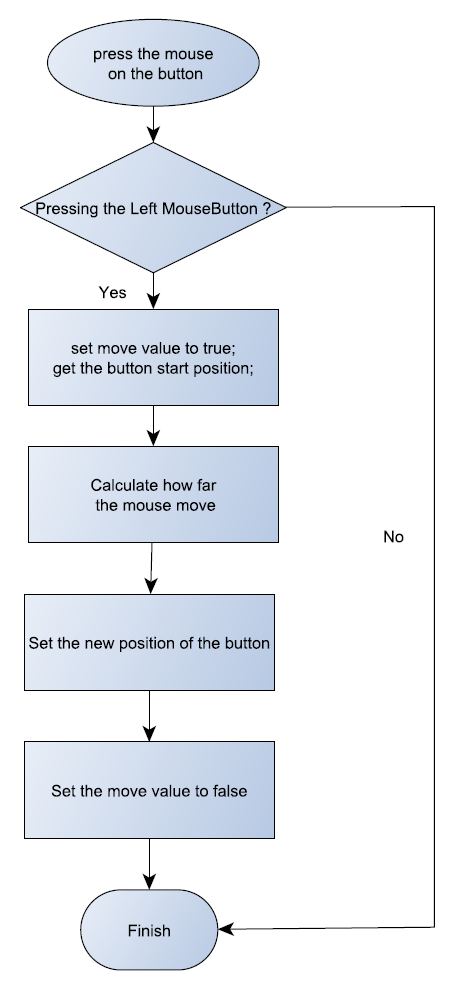
\includegraphics[width=50mm]{./Images/Software/drag_button_on_panel.png}
		\caption{Drag node move on the panel design of IDE}
		\label{drag_button_on_panel}
	\end{center}
\end{figure}
\subsubsection*{create JSON and subJSON string design}
\noindent
Before trying to create a JSON string, there is one thing that needs to be done, sorting all the items in the PaintItem list<>, add nodes into the unitNameList<>, add straight lines into the straightLineNameList<>. Add curve lines into curveLineNameList<>, and also make sure all the units in order depend on their coordinate by using Sort() method. Until now it is time to create the first JSON object, json1, set the checkMark value equal to false. The checkMark is used to check whether the straight line is the last straight line or not.
 The first thing that needs to be done is to check how many straight lines in the straightLineNameList<>, if there is no straight line, call CreateSubJsonString() function to create a subJSON string which is the callBack string and add this sub string to json1. If there are lines in the straightLineNameList<>, create another JSON object json2, find the last line in the list. Compare the coordinate with all the units in the unitNameList<>, if the unit's coordinate is equal to the line's startPoint, then add the unit name to json2 and also add json2 to json1,set the checkMark equal to true. Now compare all the unit's coordinate with the last line's endPoint and do the same thing as the startPoint, but set checkMark to false. Then use the foreach function to create json string for all the unit that left in the unitNameList<>.
 The flowchart that in fig \ref{Generate_Json_string} is the flowchart design for the create JSON string and subJSON string.
\begin{figure}[!ht]
	\begin{center}
		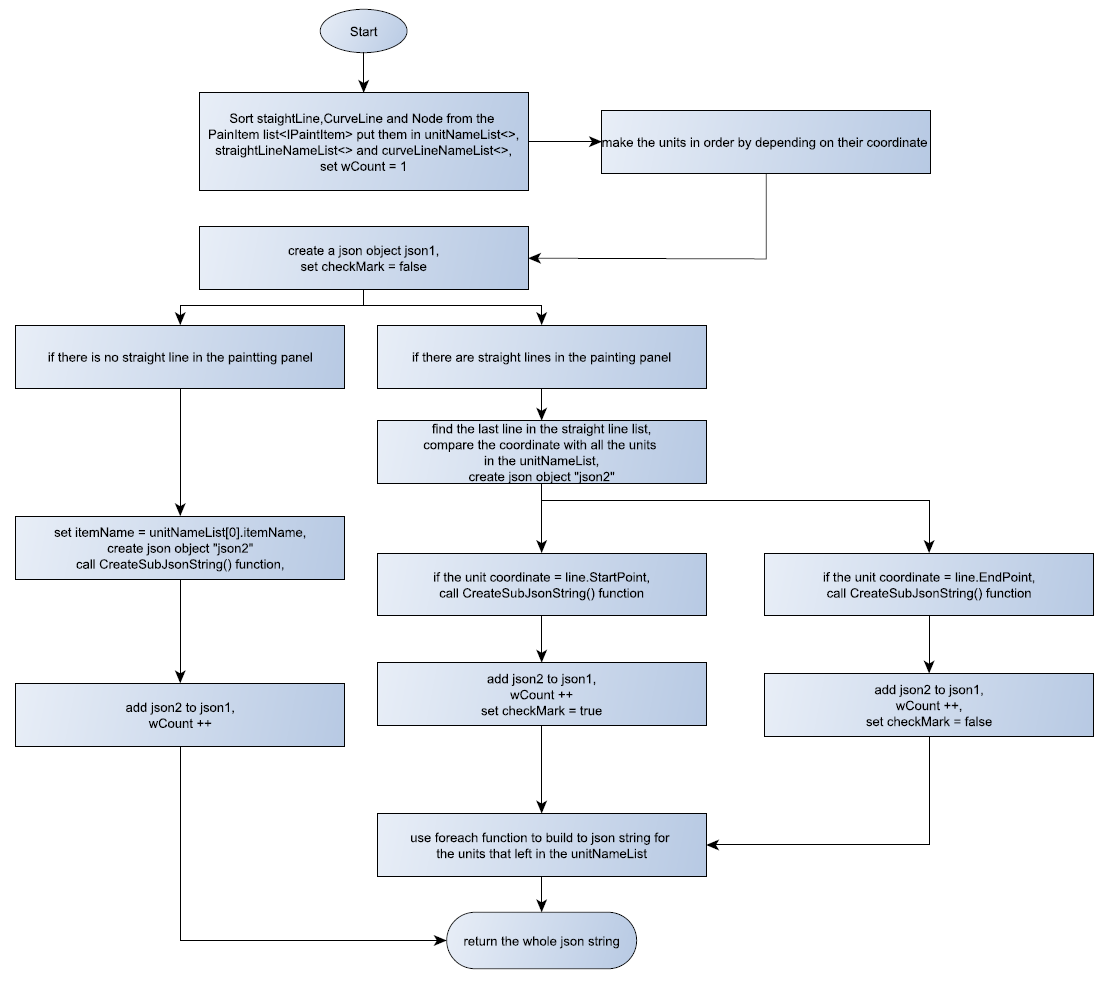
\includegraphics[width=80mm]{./Images/Software/Generate_Json_string.png}
		\caption{Create json string design of IDE}
		\label{Generate_Json_string}
	\end{center}
\end{figure}
\begin{figure}[!ht]
	\begin{center}
		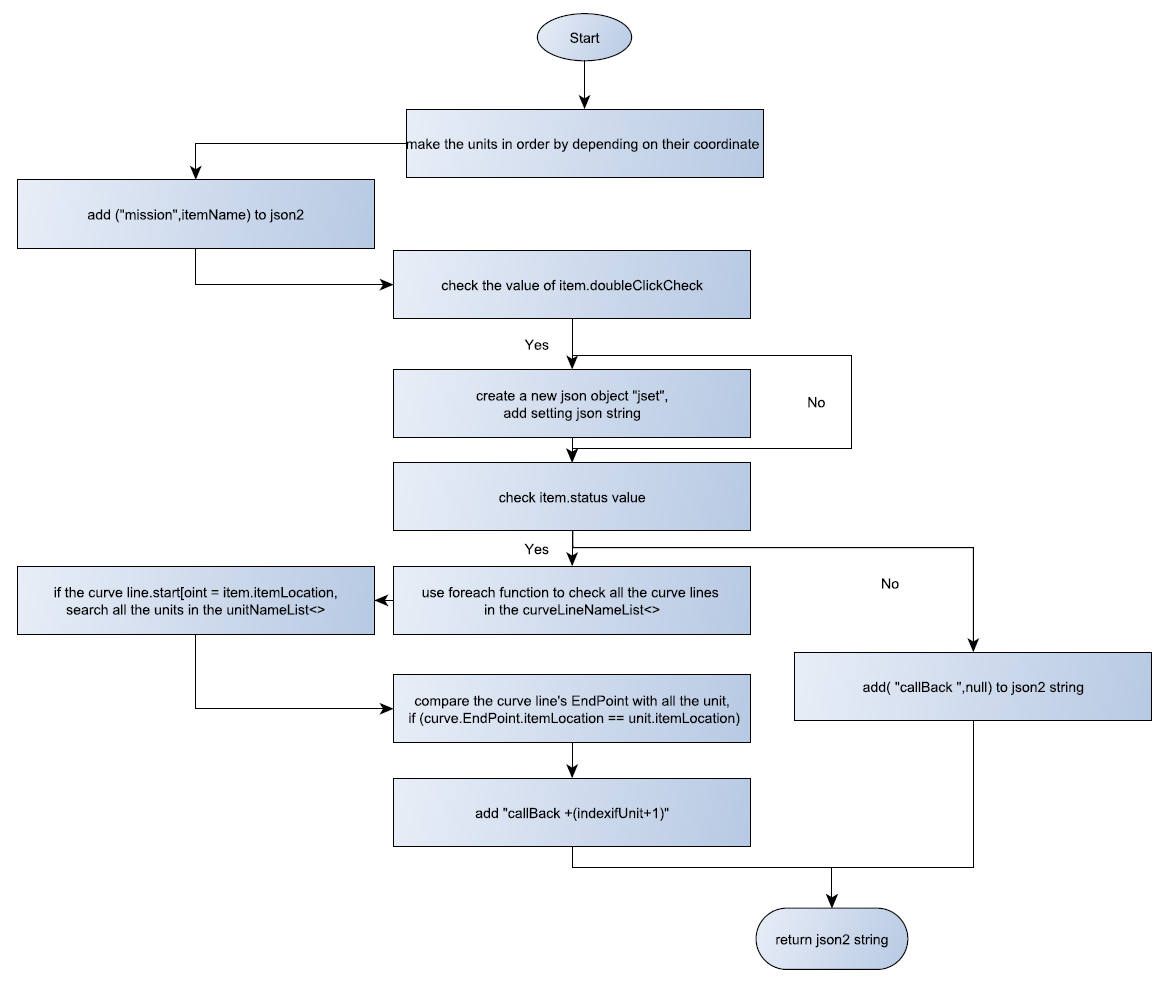
\includegraphics[width=80mm]{./Images/Software/Generate_SubJson_string.png}
		\caption{Create sub json string design of IDE}
		\label{Generate_SubJson_string}
	\end{center}
\end{figure}

\subsubsection*{PID control design}
\noindent
There are three parts on the PID control panel, the position control part, the orientation control part and the TCP communication part. The user can set the value for P,I,D from position x, position y and position z in the position control. From the orientation part the user can set the PID values for yaw, pitch and roll. When the values are set, the user can type enter the IP address and port number and then send the value to BBB. Since there are a lot of values to be set, there is a save and an import button which will make it easier for the user in not having to input all values every time. 
\subsubsection*{CAN message setting design}
\noindent
In this panel, user can set the ID of the CAN message and also the value of the message, after this the programme can figure out the length of the message and display number on the screen. When the user type into the IP-address and port number and press the send button, the message will be send to Naiad.

In appendix \ref{interface} the different functions of the GUI is described in further detail. 
	\subsubsection{Simulation} %Joakim
	\subsubsection*{Modes}
		\noindent
		The simulation node can be set in two different modes.
		\begin{itemize}
  			\item Simulation mode
  			\item IMU mode
		\end{itemize}
	\subsubsection*{Simulation mode}
		\noindent
		In simulation mode a virtual simulated representation of the Naiad robot is run with simulated sensors and actuators. The simulation allows you to be connected directly to the PID controller through TCP sockets, sending equal data as the real sensor node would have done if the robot was running a real task and receiving the real motor values that the PID controller would send to the real robot. These motor values are turned into estimated forces that is shown as dynamic lines coming from the different motor positions to give a good visualization of the forces that is acting on the robot.
		
		The calculations done in the simulation is based on the physical entities of the robot in order to get as accurate estimations of the forces that are acting on the robot as possible.
		
		By converting the motor values from the PID controller into estimated forces its possible to use these forces in the Newtonian equations to get an estimation of the translation of the robot and motion of inertia equations to estimate the orientation of the robot.
		
		Based on Newtons second law of motion the translational and orientational acceleration can be determined by the equations \ref{sim_pic1} and \ref{sim_pic2}.
		
		\begin{center}
		\begin{figure}[!ht]
		\begin{equation}\label{sim_pic1}
		F=m*a		
		\end{equation}	
		\caption{Base equation to get the linear motion}
		\begin{equation}\label{sim_pic2}
		\tau =I\alpha
		\end{equation}
		\caption{Base equation to get the rotational motion}
		\end{figure}
		\end{center}
		


\begin{center}
\begin{figure}[!ht]
\begin{equation}
\left(
\begin{array}{cccccc}
0.866025 & 0.5 & 0.0 & 0.0 & 0.0 & 0.28\\ 
0.0 & 1.0 & 0.0 & 0.0 & 0.0 & 0.22\\ 
0.866025 & -0.5 & 0.0 & 0.0 & 0.0 & -0.28\\ 
0.0 & 0.0 & 1.0 & 0.355 & 0.230 & 0.0\\ 
0.0 & 0.0 & 1.0 & -0.355 & 0.230 & 0.0\\ 
0.0 & 0.0 & 1.0 & 0.0 & -0.355 & 0.0
\end{array}
\right)
\end{equation}
\caption{\label{ThrusterConfig}Thruster configuration matrix}
\end{figure}
\end{center}

Combined with the Newtonian equations a thruster configuration matrix, found in fig. \ref{ThrusterConfig} was used that is based on the distances and angles of each motor relative to Naiads center of gravity (COG) that makes the motion calculations less computationally heavy and easier to edit.
Each row in the thruster configuration matrix represent the corresponding motors motion components. The first three columns represent the X, Y and Z translational component and the last three columns represents the Roll, Pitch and Yaw rotational components.

\begin{figure}[!ht]
\begin{center}
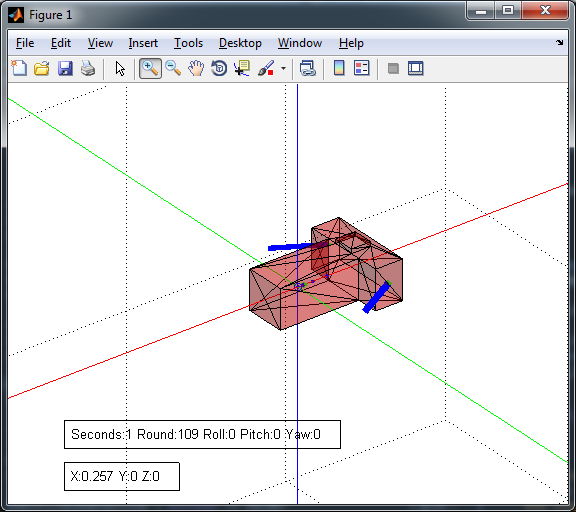
\includegraphics[width=80mm]{./Images/Software/simforward.png}
\caption{Visual representation of Naiad and forces while running in simulation mode}
\label{simforward}
\end{center}
\end{figure}

To make an accurate estimation of the time varying local coordinate frame that the robot would be in after the forces have acted on the body a rotation matrix is determined by the equations \ref{sim_eq1}-\ref{sim_eq2}\cite{petercorke}.


\begin{figure}[!ht]
\begin{center}
\begin{equation}
R^{'}(t)=S(\omega)R(t)
\label{sim_eq1}
\end{equation}
and,
\begin{equation}
R(t+\delta _{t})\approx \delta _{t}R^{'}+R(t)
\end{equation}
which can be combined to,
\begin{equation}
R(t+\delta _{t})\approx \delta _{t}S(\omega )R(t)+R(t)
\label{sim_eq2}
\end{equation}
\end{center}
\end{figure}

Where S is a skew-symmetric matrix that contains the angular velocities that is integrated from the angular accelerations determined by the Newtonian equations.
		
	\subsubsection*{IMU mode}
In IMU mode the simulator can be set into a passive mode that shows a virtual visual representation of the estimated position and orientation that the system in real time has estimated.
No calculations is needed in this mode more than rotating the virtual robot in the right order.